%
% File emnlp2016.tex
%

\documentclass[11pt,letterpaper]{article}
\usepackage{emnlp2016}		
\usepackage{times}
\usepackage{latexsym}

\usepackage{amsmath}
\usepackage{fancyvrb, fancyhdr, theorem, latexsym, color, longtable}
\usepackage{multirow}
\usepackage{url}
\usepackage{bm}
\usepackage{amssymb}

\usepackage{fixltx2e}
\usepackage{tabularx}
\usepackage{hyperref}
\usepackage{graphicx}

%\usepackage{algorithm}% http://ctan.org/pkg/algorithms
%\usepackage{algpseudocode}% http://ctan.org/pkg/algorithmicx

%\usepackage[algo2e,lined]{algorithm2e}
%\usepackage{algorithm}
%\usepackage{algorithmic}

\usepackage{color}
\newcommand{\todo}[1]{\textcolor{red}{TODO: #1}}
\newcommand{\note}[1]{\textcolor{red}{#1}}
\newcommand{\svmr}{{SVM$^{rank}$}}
\newcommand{\code}[1]{{\tt {\small #1}}}
\newcommand{\qn}{{{\bf Q}$^\textbf{{\small N}}$}}
\newcommand{\ssa}{{{\scriptsize $^{*}$}}}


\DeclareMathOperator*{\argmax}{arg\,max}
%\setlength\titlebox{6.5cm}    % Expanding the titlebox


% Uncomment this line for the final submission:
\emnlpfinalcopy

%  Enter the EMNLP Paper ID here:
\def\emnlppaperid{392}

% To expand the titlebox for more authors, uncomment
% below and set accordingly.
% \addtolength\titlebox{.5in}    

\newcommand\BibTeX{B{\sc ib}\TeX}


\title{Creating Causal Embeddings for Question Answering \\with Minimal Supervision
%\Thanks{Thanks.....}
}

% authors: Becky, Mihai, Peter, Mike, Peter C.

% Author information can be set in various styles:
% For several authors from the same institution:
\author{Rebecca Sharp, Mihai Surdeanu, Peter Jansen, Peter Clark, \and Michael Hammond \\ University of Arizona, Allen Institute for Artificial Intelligence \\ \{bsharp, msurdeanu, pajansen, hammond\}@email.arizona.edu, PeterC@allenai.org}
% if the names do not fit well on one line use
%         Author 1 \\ {\bf Author 2} \\ ... \\ {\bf Author n} \\
% For authors from different institutions:
% \author{Author 1 \\ Address line \\  ... \\ Address line
%         \And  ... \And
%         Author n \\ Address line \\ ... \\ Address line}
% To start a seperate ``row'' of authors use \AND, as in
% \author{Author 1 \\ Address line \\  ... \\ Address line
%%         \AND
%         Author 2 \\ Address line \\ ... \\ Address line \And
%         Author 3 \\ Address line \\ ... \\ Address line}
% If the title and author information does not fit in the area allocated,
% place \setlength\titlebox{<new height>} right after
% at the top, where <new height> can be something larger than 2.25in

%\author{authors\\
%  {\tt publication@emnlp2016.net}}
%\date{}



\begin{document}
\vspace{-5mm}
\maketitle

%\twocolumn[\centering \Large \bf Creating Causal Embeddings for Question Answering \\with Minimal Supervision \par
%~\\
%
%\large \bf Anonymous EMNLP submission
%~\\
%~\\
%]

\begin{abstract}
A common model for question answering (QA) is that a good answer is one that is closely related to the question, where relatedness is often determined using general-purpose lexical models such as word embeddings. 
We argue that a better approach is to look for answers that are related to the question in a {\em relevant way}, according to the information need of the question,
%We argue that a better approach is to look for answers that are related to the question in {\em the right way} \todo{"the right way" doesn't say much... Can we say something like "in a way relevant to the type of information need, or something like that?}, 
which may be determined through task-specific embeddings. 
With causality as a use case, we implement this insight in three steps. First, we generate causal embeddings cost-effectively by bootstrapping cause-effect pairs extracted from free text using a small set of seed patterns. Second, we train dedicated embeddings over this data, by using task-specific contexts, i.e., the context of a cause is its effect. Finally, we extend a state-of-the-art reranking approach for QA to incorporate these causal embeddings. We evaluate the causal embedding models both \emph{directly} with a casual implication task,
% \todo{"Word similarity" makes it sound like we do lexical similarity... Can you say something causal implication?}, 
 and \emph{indirectly}, in a downstream causal QA task using data from Yahoo! Answers. We show that explicitly modeling causality improves performance in both tasks. In the QA task our best model achieves 37.3\% P@1, significantly outperforming a strong baseline by 7.7\% (relative). 
% ms: not sure if we should discuss the differences between the 2 tasks here; we might not have space; it might dilute the message.

%
%Question answering (QA) is a difficult task, complicated by the variety of question types represented in any given question set.  In this work we propose addressing question types individually through the use of dedicated relation embeddings, and here focus on causal relations. 
%We train causal embeddings (as well as two other popular distributional similarity models) on causal tuples extracted from free text resources with minimal supervision, using a small set of high-precision patterns.   
%We evaluate these causal models both \emph{directly} in terms of their ability to detect causality, and \emph{indirectly}, in terms of their utility on a causal subset of Yahoo! Answers.
%In both tasks, we show that explicitly modeling causality significantly improves performance, and in the QA task our best model achieves 37.3\% precision at one, outperforming a strong information retrieval and lexical semantic baseline by 7.7\% (relative). 
%Importantly, we also show that the results of these two evaluations are \emph{not} identical: a given model's performance on the direct evaluation does not necessarily transfer to the more complex, real-world QA task.  
\end{abstract}



\section{Introduction}
\vspace{-2mm}

 Question Answering (QA) is a challenging task that draws upon many aspects of NLP.  Unlike search or information retrieval, answers infrequently contain lexical overlap with the question (e.g. {\em What should we eat for breakfast? -- Zoe's Diner has good pancakes}), and require QA models to draw upon more complex methods to bridge this "lexical chasm" \cite{Berger:00}.  These methods range from robust shallow models based on lexical semantics, to deeper, explainably-correct, but much more brittle inference methods based on first order logic.  

Berger et al.~\citeyear{Berger:00} proposed that this "lexical chasm" might be partially bridged by repurposing statistical machine translation (SMT) models for QA. Instead of translating text from one language to another, these monolingual alignment models learn to translate from question to answer\footnote{In practice, alignment for QA is often done from answer to question, as answers tend to be longer and provide more opportunity for association~\cite{Surdeanu:11}.}, learning common associations from question terms such as {\em eat} or {\em breakfast} to answer terms like {\em kitchen, pancakes, or cereal}.

While monolingual alignment models have enjoyed a good deal of recent success in QA (see related work), they have expensive training data requirements,  
requiring a large set of aligned in-domain question-answer pairs for training.
% ms: this footnote dilutes the message: too specific for this discussion.
%\footnote{We have empirically observed that alignment models tend to generalize better between training and test folds when the alignment model is trained on its own fold, further increasing the number of high-quality QA pairs required.}.  
%In most domains these pairs are expensive to generate, and one of the current methodological challenges in QA is locating or building high-quality QA pairs for training and testing. Even large open-domain international evaluations and workshops such as the Text REtrieval Conference (TREC)\footnote{\url{http://trec.nist.gov}} and the Cross Language Evaluation Forum (CLEF),\footnote{\url{http://www.clef-initiative.eu}} are often limited to sets of a few hundred factoid questions, many of which are highly related.  As a result, for open domain QA one often makes use of Community Question Answering (CQA) data from websites such as Yahoo! Answers or Stack Overflow, which offer tens of thousands of questions, but of highly variable quality.  
For low-resource languages or specialized domains like science or biology, often the only option is to enlist a domain expert to generate gold QA pairs --  a process that is both expensive and time consuming.  All of this means that only in rare cases are we accorded the luxury of having enough high-quality QA pairs to properly train an alignment model, and so these models are often underutilized or left struggling for resources. 

Making use of recent advancements in discourse parsing \cite{feng12}, here we address this issue, and investigate whether alignment models for QA can be trained from artificial question-answer pairs generated from discourse structures imposed on free text.
% by imposing structure on inexpensive free text resources instead of using QA pairs.  
We evaluate our methods on two corpora, generating alignment models for an open-domain  community QA task using Gigaword\footnote{LDC catalog number LDC2012T21}, and for a biology-domain QA task using a biology textbook. 

The contributions of this work are:
\begin{enumerate}
\vspace{-3mm}
\item We demonstrate that by exploiting the discourse structure of free text, monolingual alignment models can be trained to surpass the performance of models built from expensive in-domain question-answer pairs. 
\vspace{-3mm}
\item We compare two methods of discourse parsing: a simple sequential model, and a deep model based on Rhetorical Structure Theory (RST)~\cite{mann88}.  We show that the RST-based method captures within and across-sentence alignments and performs better than the sequential model, but the sequential model is an acceptable approximation when a discourse parser is not available.  
\vspace{-3mm}
\item We evaluate the proposed methods on two corpora, including a low-resource domain where training data is expensive (biology).
\vspace{-3mm}
\item We experimentally demonstrate that monolingual alignment models trained using our method considerably outperform state-of-the-art neural network language models in low resource domains.
\end{enumerate}










%the task of question answering (QA) has received considerable attention. However, most of this effort has focused on factoid questions rather than more complex non-factoid (NF) questions, such as manner, reason, or causation questions. Moreover, the vast majority of QA models explore only 
%%similarity models based on 
%local linguistic structures, such as syntactic dependencies or semantic role frames, which are generally restricted to individual sentences. This is problematic for NF QA, where questions are answered 
% not by atomic facts, but 
%by larger cross-sentence conceptual structures that convey the desired answers. Thus, to answer NF questions, one needs a model of what these answer structures look like.
%
%Driven by this observation, our main hypothesis is that the discourse structure of NF answers provides complementary information to state-of-the-art QA models that measure the similarity (either lexical and/or semantic) between question and answer. 
%We propose a novel answer reranking (AR) model that combines lexical semantics (LS) with discourse information, driven by two representations of discourse: a shallow representation centered around discourse markers and surface text information, and a deep one based on the Rhetorical Structure Theory (RST) discourse framework~\cite{mann88}.
%To the best of our knowledge, this work is the first to systematically explore within- and cross-sentence structured discourse features for NF AR. The contributions of this work are:
%\begin{enumerate}
%\vspace{-3mm}
%\item We demonstrate that modeling discourse is greatly beneficial for NF AR for two types of NF questions, manner ({\em ``how"}) and reason ({\em ``why"}), across two large datasets from different genres and domains -- one from the community question-answering (CQA) site of Yahoo! Answers\footnote{\url{http://answers.yahoo.com}}, and one from a biology textbook.  
%%Our results show statistically significant improvements of over 20\%, up to 37\% (relative) on precision at 1 (P@1) when discourse is considered. Crucially, these improvements hold even on top of state-of-the-art LS models~\cite{yih13}.
%Our results show statistically significant improvements of up to 24\% on top of state-of-the-art LS models~\cite{yih13}.
%\vspace{-3mm}
%\item We demonstrate that both shallow and deep discourse representations are useful, and, in general, their combination performs best.
%\vspace{-3mm}
%\item We show that discourse-based QA models using inter-sentence features considerably outperform single-sentence models when answers span multiple sentences.
%\vspace{-3mm}
%\item We demonstrate good domain transfer performance between these corpora, suggesting that answer discourse structures are largely independent of domain, and thus broadly applicable to NF QA. 
%\end{enumerate}
%

\section{Related Work}
\label{sec:relatedwork}

In one sense, QA systems can be described in terms of their position along a formality continuum ranging from shallow models that rely on information retrieval, lexical semantics, or alignment, to highly structured models based on first order logic (FOL).  

On the shallower end of the spectrum,  QA models can be constructed either from structured text, such as question--answer pairs, or unstructured text.  Alignment models~\cite{Berger:00,echihabi2003noisy,Soricut:06,Riezler:etal:2007,Surdeanu:11,yao2013}  require aligned question--answer pairs for training, a burden which often limits their practical usage (though Sharp et al.~\citeyear{sharp-EtAl:2015:NAACL-HLT} recently proposed a method for using the discourse structure of free text as a surrogate for this alignment structure).
Lexical semantic models such as neural-network language models~\cite{jansen14,sultan-etal:2014:TACL,yih13}, on the other hand, have the advantage of being readily constructed from free text.  
Fried et al.~\citeyear{fried2015higher} called these approaches first-order models because associations are explicitly learned, and introduced a higher-order lexical semantics QA model where indirect associations are detected through traversals of the association graph.  
Other recent efforts have applied deep learning architectures to QA to learn non-linear answer scoring functions that model lexical semantics~\cite{Iyyer2014,nips15_hermann}.
However, while lexical semantic approaches to QA have shown robust performance across a variety of tasks, a disadvantage of these methods is that, even when a correct answer is selected, there is no clear human-readable justification for that selection.   

Closer to the other end of the formality continuum, several approaches were proposed to not only select a correct answer, but also provide a formally valid justification for that answer.  For example, some QA systems have sought to answer questions by creating formal proofs driven by logic reasoning~\cite{moldovan2003cogex,moldovan2007cogex,balduccini2008knowledge,maccartney2009natural,liang2013learning,lewis2013combining}, answer-set programming \cite{baral2006using,baral2011towards,baral2012answering,baral2012knowledge}, or connecting semantic graphs~\cite{banarescu2012amr,sharmatowards}. 
However, the formal representations used in these systems, e.g., logic forms, are both expensive to generate 
and tend to be brittle because they rely extensively on imperfect tools such as complete syntactic analysis and word sense disambiguation.
We offer the lightly-structured sentence representation generated by our approach (see Section \ref{sec:tag}) as a shallower and consequently more robust approximation of those logical forms, and show that they are well-suited for the complexity of our questions.
Our approach allows us to robustly aggregate information from a variety of knowledge sources to create human-readable answer justifications.  
It is these justifications which are then ranked in order to choose the correct answer, using a reranking perceptron with a latent layer that models the correctness of those justifications.


Covering the middle ground between shallow and formal representations, learning to rank methods based on tree-kernels~\cite{Moschitti:04} perform well for various QA tasks, including passage reranking, answer sentence selection, or answer extraction~\cite[inter alia]{Moschitti:07,Moschitti:11,Severyn:12,Severyn:13a,Severyn:13b,Tymoshenko:15}. 
The key to tree kernels' success is their ability to automate feature engineering rather than having to rely on hand-crafted features, which allows them to explore a larger representation space. Further, tree kernels operate over structures that encode syntax and/or shallow semantics such as semantic role labeling~\cite{Severyn:12}, knowledge from structured databases~\cite{Tymoshenko:15}, and higher level semantic information such as question category and focus words~\cite{Severyn:13b}.
Here, we similarly use structural features based on syntax, and enriched with additional information about how the answer candidate, the question, and the aggregated justification relate to each other.  
A key difference between our work and methods based on tree kernels is that rather than selecting a contiguous segment of text (sentence or paragraph) our justifications are aggregated from multiple sentences, often from different documents. Because of this setup, we explore content representations that continue to use syntax, but combined with robust strategies for cross-sentence connections. Further, because our justification search space is increased considerably due to the ability to form cross-sentence justifications, we restrict our learning models to linear classifiers that learn efficiently at this scale. However, as discussed, tree kernels offer distinct advantages over linear models. We leave the adaptation of tree kernels to the problem discussed here as future work.



Information aggregation (or fusion) is broadly defined as the assembly of knowledge from different sources, and has been used in several NLP applications, including summarization and QA.  In the context of summarization, information aggregation has been used to assemble summaries from non-contiguous text fragments~\cite[inter alia]{barzilay1999information,barzilay2005sentence}, while in QA, aggregation has been used to assemble answers to both factoid questions~\cite{pradhan2002building} and definitional questions~\cite{blair2003hybrid}.  Critical to the current work, in an in-depth open-domain QA error analysis, Moldovan et al. \citeyear{Moldovan:2003:PIE:763693.763694} identified a subset of questions for which information from a single source is not sufficient, and designated a separate class within their taxonomy of QA systems for those systems which were capable of performing answer fusion. Combining multiple sources, however, creates the need for context disambiguation -- an issue we tackle through the use of question and answer focus words.

Identifying question focus words, a subtask of question decomposition and identifying information needs, was found relevant for QA (especially factoid) early on~\cite[inter alia]{Harabagiu:00,Moldovan:2003:PIE:763693.763694} mainly as a means to identify answer types (e.g., "What is the {\em capital} of France?" indicates the expected answer type is \emph{City}).  
Recently, Park and Croft~\citeyear{Park:2015} have used focus words to reduce semantic drift in query expansion, by conditioning on the focus words when expanding non-focus query words.
Similarly, here, we use focus words (from both question and answer) to reduce the interference of noise in both building and ranking answer justifications.  By identifying which words are most likely to be important for finding the answer, we are able to generate justifications that preferentially connect sentences together on these focus words.  This results in justifications that are better able to remain on-context, and as we demonstrate in Section \ref{sec:experiments}, this boosts overall performance. 

Once the candidate answer justifications are assembled, our method selects the answer which corresponds to the best (i.e., highest-scoring) justification.  We learn which justifications are indicative of a correct answer by extending ranking perceptrons~\cite{Shen:Joshi:2005}, which have been previously used in QA~\cite{Surdeanu:11}, to include a latent layer that models the correctness of the justifications. Latent-variable perceptrons have been proposed for several other NLP tasks~\cite{liang2006end,zettlemoyer2007online,sun2009latent,hoffmann2011knowledge,fernandes2012latent,bjorkelund2014learning}, but to our knowledge, we are the first to adapt them to reranking scenarios. 

Finally, we round out our discussion of question answering systems with a comparison to the famous Watson QA system, which achieved performance on par with the human champions in the Jeopardy! game~\cite{Ferucci:12}.
Several of the ideas proposed in our work are reminiscent of Watson. 
For example, our component that generates text aggregation graphs (Section 5) shares functionality with the Prismatic engine used in Watson. Similar to Watson, we extract evidence from multiple knowledge bases. However, there are three fundamental differences between Watson and this work. 
First, while Watson includes components for evidence gathering and scoring (we call these justifications), it uses a fundamentally different strategy for evidence generation. Similar to most previous work, the textual evidence extracted by Watson always takes the form of a contiguous segment of text~\cite{murdock2012textual},\footnote{Watson also generates ``structured evidence'' which is obtained by converting texts to structured representations similar to logic forms, which are then matched against structured databases for answer extraction. However, this ``logical representation of a clue and then finding the identical representation'' in a database resulted in ``confident answers less than 2\% of the time''~\cite{Ferucci:12}.} whereas our justifications aggregate texts from different documents or knowledge bases. We demonstrate in this work that information aggregation from multiple knowledge bases is fundamental for answering the science exam questions that are our focus (Section 8). 
Second, our answer ranking approach jointly ranks candidate answers and their justifications using a latent-variable learning algorithm, whereas Watson follows a pipeline approach where first evidence is generated, then answers are ranked~\cite{gondek2012framework}. We show in Section 8 that jointly learning answers and their justifications is beneficial. 
Last but not least, Watson was implemented as a combination of distinct models triggered by the different types of Jeopardy! questions, whereas our approach deploys a single model for all questions. Our analysis in Section~\ref{sec:erroranalysis} suggests that there are limits to our simple approach: we measure a ceiling performance for our single-model approach of approximately 70\%. To surpass this ceiling, one would have to  implemented dedicated domain-specific methods for the difficult problems left unsolved by our approach. 



\begin{figure}[t]
\begin{center}
\includegraphics[width=0.3\textwidth]{arch_overall.png}
\caption{ Architecture of our question answering approach.  
Given a question, candidate answer, and a free-text knowledge base as inputs, we generate a pool of candidate justifications, from which we extract feature vectors.  We use a neural network to score each and then use max-pooling to select the current best justification. This serves as the score for the candidate answer itself.  The red border indicates the components that are trained online. }
\label{fig:arch_overall}
\vspace{-5mm}
\end{center}
\end{figure}

\section{Approach}
\label{sec:approach}
One of the primary difficulties with the explainable QA task addressed here is that, while we have supervision for the correct answer, we do not have annotated answer justifications.  
Here we tackle this challenge by using the QA task performance as supervision for the justification reranking, allowing us to 
%extending a neural QA model to jointly learn both how to 
%jointly 
learn to choose both the correct answer and a compelling, human-readable justification for that answer.

Additionally, similar to the strategy Chen and Manning~\shortcite{chen2014fast} applied to parsing, we combine representation-based features with explicit features that capture additional information that is difficult to model through embeddings, especially with limited training data.
%second contribution is that, similar to the strategy Chen and Manning~\shortcite{chen2014fast} applied to parsing, we combine representation-based features with explicit features that capture additional information that is difficult to model through embeddings.



% ms: avoid "system" too engineering-y
The architecture of our approach is summarized in Figure \ref{fig:arch_overall}.  
Given a question and a candidate answer, we first query an textual knowledge base (KB) to retrieve a pool of potential justifications for that answer candidate.  
For each justification, we extract a set of features designed to model the relations between questions, answers, and answer justifications based on word embeddings, lexical overlap with the question and answer candidate, discourse, and information retrieval (IR) (Section \ref{sec:features}).
These features are passed into a simple neural network to generate a score for each justification, given the current state of the model.  A final max-pooling layer selects the top-scoring justification for the candidate answer and this max score is used also as the score for the answer candidate.  
The system is trained using correct-incorrect answer pairs with a pairwise margin ranking loss objective function to enforce that the correct answer be ranked higher than any of the incorrect answers. 

%The key here is that we use the current state of the model to select the best justification for a given answer candidate from a pool of many candidate justifications.  To do this, we modify the training procedure such that at the start of each epoch \todo{minibatch instead of epoch?}, we first compute a forward pass with each candidate justification to find the top-scoring justification for each candidate answer.
%For a given question, answer candidate, and justification, we combine features based on word embeddings, lexical overlap, discourse, and information retrieval (IR) together in a simple neural architecture to generate a score for the answer candidate.    We then use this selected justification to calculate our gradients for updating the model parameters.  

With this end-to-end approach, the model learns to select justifications that allow it to correctly answer questions.  We hypothesize that this approach enables the model to indirectly learn to choose justifications that provide good explanations as to why the answer is correct. We empirically test this hypothesis in Section \ref{sec:results}, where we show that indeed the model learns to correctly answer questions, as well as to select high-quality justifications for those answers. 
% ms: misleading; it reads as if answer selection is better than IR
% better than a strong IR baseline. 


\section{Extracting Cause-Effect Tuples}
\label{sec:causalextraction}
%\vspace{-2mm}

%Information extraction (IE) systems which are designed to extract events typically make use of either machine learning (ML) or hand-built rules or patterns.  %IE classifiers which use ML are generally considered to be either fully supervised (trained only on annotated data), semi-supervised (trained on a combination of labelled data and the data which is bootstrapped from it or by using a large database of pre-known event tuples), or unsupervised (when no labelled data is available for training).
%For causal events, we have neither labelled data nor an existing, large database of cause-effect pairs from which we could use ML to train a supervised or semi-supervised classifier.  Additionally, while unsupervised or distant supervision approaches are well-suited to situations where the desired event types and the patterns that would identify them are unknown, here we know exactly what relation we want (causality) and the patterns needed to find these events are relatively explicit.  For these reasons, we opted to use boostrapping to extract a large number of cause-effect pairs from a small set of patterns.

Because the success of embedding models depends on large training datasets \cite{sharp2015spinning}, and such datasets do not exist for open-domain causality, we opted to bootstrap a large number of cause-effect pairs from a small set of patterns.
%
We wrote these patterns using Odin~\cite{valenzuela2016runes}, a rule-based information extraction framework which has the distinct advantage of 
being able to operate over multiple representations of content (i.e., surface and syntax).
%being \emph{expressive}.  That is, while most open-source rule languages operate over one representation of text (e.g., GATE~\cite{Cunningham2011a} generally operates over surface sequences, whereas Semgrex~\cite{chambers2007learning} operates over syntactic dependencies), Odin has the flexibility to use either (or both) depending on the user's need.  
For this work, we make use of rules that operate over both surface sequences as well as dependency syntax in the grammars introduced in steps (2) and (3) below.

Odin operates as a cascade, % of grammars, 
allowing us to implement a two-stage approach.
%. Taking advantage of this architecture, we implemented a two-stage approach.
First, we identify potential participants in causal relations, i.e., the potential causes and effects, which we term {\bf causal mentions (CM)}. A second grammar then identifies actual causal relations that take these CMs as arguments.

We consider both noun phrases (NP) as well as entire %non-causal
clauses to be potential CMs, since causal patterns form around participants that are syntactically more complex than flat NPs.  
%For example, in the sentence \emph{The hurricane caused significant damage}, both the cause ({\em hurricane}) and effect ({\em damage}) are non-recursive noun phrases.  On the other hand, 
For example, in the sentence \emph{The collapse of the housing bubble caused stock prices to fall}, both the cause ({\em the collapse of the housing bubble}) and effect ({\em stock prices to fall}) are more complicated nested structures.  Reducing these arguments to non-recursive NPs (e.g., {\em The collapse} and {\em stock prices}) is clearly insufficient to capture the relevant context.

%Examples of the rules to extract CMs as well as causal events are shown in Table \ref{tab:rule_examples}\todo{rule examples table}, 

%\begin{table}[t!]
%\begin{center}
%%\begin{scriptsize}
%\begin{footnotesize}
%\begin{tabular}{ll}
%\hline
%\multicolumn{1}{l}{ Rule } & \multicolumn{1}{l}{Example Sentence} \\ %\multicolumn{1}{l}{Impr.} \\
%%\cline{1-2}
%
%\hline
%%\multicolumn{2}{l}{\textit{Yahoo! Answers}} \\ % 185q (sent) ret=1p c=0.1 
%%\hline
%			  &  	\\
%			& 	\\
%	  		& 	\\
%			& 	\\
%
%\end{tabular}
%\end{footnotesize}
%\caption{{\small caption}}
%\label{tab:rules}
%\end{center}
%\end{table}



Formally, we extract our causal relations using the following algorithm:
{\flushleft \textbf{(1) Pre-processing:}} Much of the text we use to extract causal relation tuples comes from the Annotated Gigaword \cite{napoles2012annotated}.  This text is already fully annotated and no further processing is necessary.  We additionally use text from the Simple English Wikipedia\footnote{{\scriptsize \url{https://simple.wikipedia.org/wiki/Main_Page}}.  The Simple English version was preferred over the full version due to its simpler sentence structures, which make extracting cause-effect tuples more straightforward.}, which we processed using the Stanford CoreNLP toolkit~\cite{Manning:14} and the dependency parser of Chen and Manning~\citeyear{chen14}.

{\flushleft \textbf{(2) CM identification:}} \label{step:cm} We extract causal mentions (which are able to serve as arguments in our causal patterns) using a set of rules % (shown in Table \ref{tab:cm_rules}) 
designed to be robust to the variety that exists in natural language. %, and therefore in the dependency parses.  
Namely, to find CMs that are noun phrases, we first find words that are tagged as nouns, then follow outgoing dependency links for modifiers and attached prepositional phrases\footnote{The outgoing dependency links from the nouns which we followed were: \texttt{nn, amod, advmod, ccmod, dobj, prep\_of, prep\_with, prep\_for, prep\_into, prep\_on, prep\_to}, and \texttt{prep\_in}.}, to a maximum depth of two links.  To find CMs that are clauses, we first find words that are tagged as verbs (excluding verbs which themselves were considered to signal causation\footnote{The verbs we excluded were: \emph{cause, result, lead, create}.}), then again follow outgoing dependency links for modifiers and arguments.  We used a total of four rules to label CMs.%\footnote{The two complete grammars, for both CM and causal relation identification, were submitted as supplemental material. \todo{This is no longer relevant. Please remove.}}
%There were a total of four rules used to label CMs, and examples are shown in Table~\ref{tab:rules}.

{\flushleft \textbf{(3) Causal tuple extraction:}} \label{step:causalext} After CMs are identified, a grammar scans the text for causal relations that have CMs as arguments.  Different patterns have varying probabilities of signaling causation~\cite{khoo1998automatic}.  To minimize the noise in the extracted pairs, we restrict ourselves to a set of 13 rules designed to find unambiguously causal patterns, such as {\em CAUSE led to EFFECT}, where {\em CAUSE} and {\em EFFECT} are CMs.
The rules operate by looking for a \emph{trigger} phrase, e.g., {\em led}, and then following the dependency paths to and/or from the trigger phrase to see if all required CM arguments exist.
%, which tells the rule to fire.  Once a trigger is found, the rule follows the dependency paths to and/or from the trigger phrase to see if all specified arguments exist, e.g.,  following an outgoing {\tt nsubj} to identify the cause in the previous example.
%An example of this is shown in Figure \ref{fig:rule_ex}. Here, when the rule scans the sentence \emph{SENTENCE TEXT}, the trigger verb \emph{cause} is found, then the rule checks for an outgoing \texttt{nsubj} dependency link and an outgoing \texttt{dobj} link to previously found CMs.  
%%Our grammars also ensure that the triggers are not negated (we used Odin lookaround assertions to check that outgoing \texttt{neg} dependencies are not attached to triggers).  % Since in this example, all conditions are met, the rule returns the causal event in the form of the tuple (\todo{example}).

% ms: removed for space
%At step~2, the identification of CMs, we place few restrictions on the CM syntactic subgraph, favoring recall since in step 3 we use high-precision rules.  The rule set for step \ref{step:causalext}, in fact, was winnowed down after early experiments showed that many patterns which \emph{can} indicate causation (e.g., {\em X happened due to Y}) often are non-causal (\todo{example}).  

\begin{table}[t!]
\begin{center}
%\begin{scriptsize}
\begin{footnotesize}
\begin{tabular}{lc}
\hline
Corpus		&	Extracted Tuples		 \\
\hline
%\multicolumn{2}{l}{\textit{Yahoo! Answers}} \\ % 185q (sent) ret=1p c=0.1 
%\hline
Annotated Gigaword	& 798,808 	\\
Simple English Wikipedia		& 16,425 	\\
\hline
Total		& 815,233 	\\
\end{tabular}
\end{footnotesize}
\caption{{\footnotesize Number of causal tuples extracted from each corpus.}} 
\label{tab:causalstats}
\vspace{-4mm}
\end{center}
\end{table}

%ltw_mar30_combo.argsC: 55882
%nyt_mar30_combo.argsC: 260460
%wpb_mar30_combo.argsC: 7522
%apw_mar30_combo.argsC: 219348
%xin_mar30_combo.argsC: 76183
%simpleWiki_mar19b_combo.argsC: 14057
%cna_mar30_combo.argsC: 7913
%afp_mar30_combo.argsC: 133003
%sum: 774368

Applying this causal grammar over Gigaword and Simple English Wikipedia produced %774,368 casual tuples, after stop-word and part-of-speech filtering.
815,233 causal tuples, as summarized in Table~\ref{tab:causalstats}. As bootstrapping methods are typically noisy, we manually evaluated the quality of approximately 250 of these pairs selected at random.  Of the tuples evaluated, approximately 44\% contained some amount of noise. For example, from the sentence \emph{Except for Springer's show, which still relies heavily on confrontational topics that lead to fistfights virtually every day...}, while ideally we would only extract (\emph{confrontational topics $\rightarrow$ fistfights}), instead we extract the tuple (\emph{show which still relies heavily on confrontational topics} $\rightarrow$ \emph{fistfights virtually every day}), which contains a large amount of noise: \emph{show, relies, heavily}, etc.
%\todo{Add one example here that is approximately wrong, that is, has some causality but is not ideal. This is to emphasize that, minimally, our tuples capture dist. sim.} 
This finding prompted our noise-aware model described at the end of Section~\ref{sec:models}.

%While this limiting of the rules greatly improved the quality of the extracted causal events, there is still a considerable amount of noise in the data -- a problem we discuss and address in Section \ref{sec:noise} \todo{noise section}. 



\section{Models}
\label{sec-emnlp2016:models}

We use the extracted causal tuples to train three distinct distributional similarity models that explicitly capture causality. 

{\flushleft \textbf{Causal Embedding Model (cEmbed):}}
The first distributional similarity model we use is based on the skip-gram word-embedding algorithm of Mikolov et al.~\citeyear{mikolov2013distributed}, which has been shown to improve a variety of language processing tasks % \footnote{Chris Manning recently called embedding models the Sriracha sauce of NLP.} 
including QA~\cite{yih13,fried2015higher}.  In particular, we use the variant implemented by Levy and Goldberg~\citeyear{levy2014dependency} which modifies the original algorithm to use an arbitrary, rather than linear, context. 
Our novel contribution is to make this context task-specific: intuitively, the context of a cause is its effect. Further, these contexts are generated from tuples that are themselves bootstrapped, which minimizes the amount of supervision necessary.

The Levy and Goldberg model trains using single-word pairs, while our CMs could be composed of multiple words.  
For this reason, we decompose each cause--effect tuple, $(CM_c,CM_e)$, such that each word $w_c \in CM_c$ is paired with each word $w_e \in CM_e$. 

%so we decompose each cause--effect tuple, $(CM_c,CM_e)$, where each CM could be multi-word, into the Cartesian product of the words in CMs. such that each $w_c \in CM_c$ has as its context all $w_e \in CM_e$. 
After filtering the extracted cause-effect tuples for stop words and retaining only nouns, verbs, and adjectives, we generated over 3.6M $(w_c, w_e)$ word-pairs\footnote{For all models proposed in this section we used lemmas rather than words.} from the approximately 800K causal tuples.

The model learns two embedding vectors for each word, one for when the word serves as a target word and another for when the word serves as a context word.  Here, since the relation of interest is inherently directional, both sets of embeddings are meaningful, and so we make use of both -- the target vectors encode the effects of given causes, whereas the context vectors capture the causes of the corresponding effects. 


{\flushleft \textbf{Causal Alignment Model (cAlign):}}
Monolingual alignment (or translation) models have been shown to be successful in QA \cite{Berger:00,Echihabi:03,Soricut:06,Riezler:etal:2007,Surdeanu:11,yao2013}, and recent work has shown that they can be successfully trained with less data than embedding models~\cite{sharp2015spinning}. 
% Further, Fried et al.~\citeyear{fried2015higher} demonstrated that \todo{dest. distribution as semantic model of the source concept, which is important for our task as well.} % ms: nice, but no space

To verify these observations in our context, we train an alignment model that ``translates'' causes (i.e., the ``source language'') into effects (i.e., the ``destination language''), using our cause--effect tuples. 
This is done using IBM Model 1~\cite{Brown:93} and GIZA++~\cite{och03}. 
%We train an alignment model from our cause--effect tuples using  IBM Model 1~\cite{Brown:93} and GIZA++~\cite{och03}.


\begin{figure}[t!]
\begin{center}
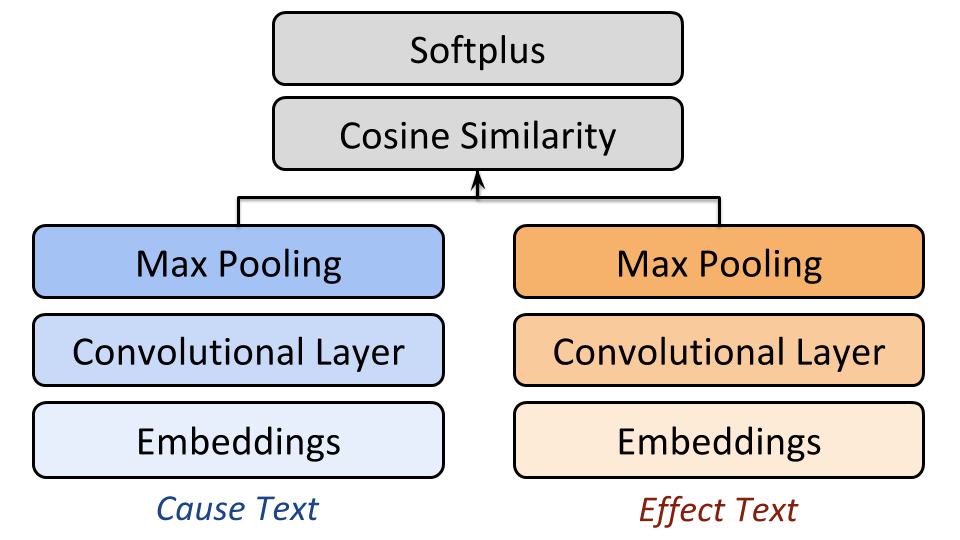
\includegraphics[width=0.7\textwidth]{mainmatter/emnlp2016-causal/cnn2.png}
%space{-2mm}
\caption{{\footnotesize Architecture of the causal convolutional network. }}
%space{-6mm}
\label{fig:cnn}
\end{center}
\end{figure}

{\flushleft \textbf{Causal Convolutional Neural Network Model (cCNN):}}
Each of the previous models have at their root a bag-of-words representation, which is a simplification of the causality task. To address this potential limitation, we additionally trained a convolutional neural network (CNN) which operates over variable-length texts, and maintains distinct embeddings for causes and effects.  The architecture of this approach is shown in Figure~\ref{fig:cnn}, and consists of two sub-networks (one for cause text and one for effect text), each of which begins by converting the corresponding text 
% (which has been padded to be of equal  length)  % ms: skip for now, until we understand it better
into 50-dimensional embeddings.  These are then fed to a convolutional layer,\footnote{The convolutional layer contained 100 filters, had a filter length of 2 (i.e., capturing bigram information), and an inner ReLU activation.} which is followed by a max-pooling layer of equal length.
Then, these top sub-network layers, which can be thought of as a type of phrasal embedding, are merged by taking their cosine similarity.  Finally, this cosine similarity is normalized by feeding it into a dense layer with a single node which has a softplus activation.  
In designing our CNN, we attempted to minimize architectural and hyperparameter tuning by taking inspiration from Iyyer et al.~\citeyear{iyyer2015deep}, preferring simpler architectures.
We train the network using a binary cross entropy objective function and the Adam optimizer~\cite{kingma2014adam}, using the Keras library~\cite{chollet2015keras} operating over Theano~\cite{2016arXiv160502688short}, a popular deep-learning framework.\footnote{We also experimented with an equivalent architecture where the sub-networks are implemented using long short-term memory (LSTM) networks~\cite{hochreiter1997long}, and found that they consistently under-perform this CNN architecture. Our conjecture is that CNNs perform better because LSTMs are more sensitive to overall word order than CNNs, which capture only local contexts, and we have relatively little training data, which prevents the LSTMs from generalizing well.}

{\flushleft \textbf{Noise-aware Causal Embedding Model (cEmbedNoise):}} 
We designed a variant of our cEmbed approach to address the potential impact of the noise introduced by our bootstrapping method.
While training, we weigh the causal tuples by the likelihood that they are truly causal, which we approximate with pointwise mutual information (PMI).
For this, we first score the tuples by their causal PMI and then scale these scores by the overall frequency of the tuple~\cite{riloff1996automatically}, to account for the PMI bias toward low-frequency items.  That is, the score $S$ of a tuple, $t$, is computed as: 

%space{-2mm}
%\scalebox{1.0}{
\begin{small}
\begin{equation}
S(t) = \log \frac{p(tuple|causal)}{p(tuple)} * \log (freq(tuple))
\end{equation} 
\end{small}
%}
%space{-2mm}

%Riloff~\citeyear{riloff1996automatically} propose a method for ranking their extracted patterns using $relevance\_rate * \log_2 (frequency)$.  As our relevance rate we use the pointwise mutual information of the extracted tuples, or $\log \frac{p(tuple|causal)}{p(tuple)}$, where $p(tuple| causal)$ is the ratio of the number of times that a given tuple is found in a causal construction versus any construction, and $p(tuple)$ is the frequency of the given tuple divided by the frequency of all the tuples. 
%Scaling the PMI by the frequency of the tuple mitigates its bias towards low-frequency items.
%we combine PMI with frequency information, so that we consider the likelihood of a pair to be causal to be:
%$p(causal|pair)$ \cite{riloff1996automatically}.
We then discretize these scores into five quantiles, ascribing a linearly decreasing weight during training to datums in lower scoring quantiles.%\footnote{\textcolor{blue}{We implemented this weighing process by repeating higher weight training examples more times.}}



\section{Direct Evaluation: Ranking Word Pairs}

\begin{figure*}[th!]
\begin{center}
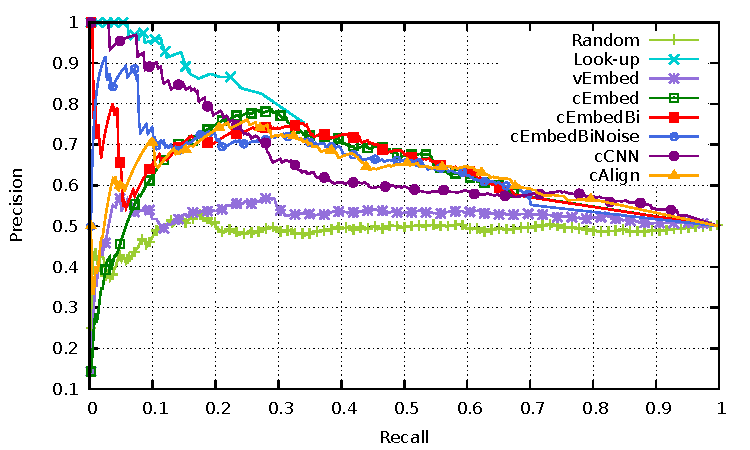
\includegraphics[width=\textwidth]{mainmatter/emnlp2016-causal/direct2.pdf} % {rpcurves_all.png}
%space{-3mm}
\caption{{\footnotesize Precision-recall curve showing the ability of each model to rank causal pairs above non-causal pairs. For clarity, we do not plot cEmbedNoise, which performs worse than cEmbedBiNoise. The Look-up model has no data points beyond the 35\% recall point.}}
%space{-4mm}
\label{fig:rpcurve_all}
\end{center}
\end{figure*}

%\flushleft{\textbf{Results:}} 

\label{sec-emnlp2016:directeval}

%Before we discuss the utility of these models for causal QA, we implement a {\em direct} evaluation
We begin the assessment of our models with a {\em direct} evaluation to determine whether or not the proposed approaches capture causality better than general-purpose word embeddings and whether their robustness improves upon a simple database look-up.
For this evaluation, we follow the protocol of Levy and Goldberg~\citeyear{levy2014dependency}.  
In particular, we create a collection of word pairs, half of which are causally related, with the other half consisting of other relations. 
These pairs are then ranked by our models and several baselines, with the goal of ranking the causal pairs above the others. 
The embedding models rank the pairs using the cosine similarity between the target vector for the causal word and the context vector of the effect word.  The alignment model ranks pairs using the probability $P(\text{Effect}|\text{Cause})$ given by IBM Model 1, and the CNN ranks pairs by the value of the output returned by the network.
%To demonstrate that their embeddings encoded functional similarity rather than relatedness, they ranked a set of word pairs (each of which reflected one of the two types of similarity) using cosine similarity and showed that the word pairs which were functionally similar tended to be ranked higher than those with topical similarity.  Here, we do the same.

%\flushleft{\textbf{Data:}} 
\subsection{Data}
In order to avoid bias towards our extraction methods, we evaluate our models on an external set of word pairs drawn from the SemEval 2010 Task 8 \cite{hendrickx2009semeval}, originally a multi-way classification of semantic relations between nominals.  We used a total of 1730 nominal pairs, 865 of which were from the Cause-Effect relation (e.g., (\emph{dancing $\rightarrow$ happiness})) and an equal number which were randomly selected from the other eight relations (e.g., (\emph{juice $\rightarrow$ grapefruit}), from the Entity-Origin relation).  This set was then randomly divided into equally-sized development and test partitions.

%\flushleft{\textbf{Baselines:}} 
\subsection{Baselines}
We compared our distributional similarity models against three baselines:

{\flushleft \textbf{Vanilla Embeddings Model (vEmbed):}} a standard \texttt{word2vec} model trained with the skip-gram algorithm and a sliding window of 5, using the original texts from which our causal pairs were extracted.\footnote{All embedding models analyzed here, including this baseline and our causal variants, produced embedding vectors of 200 dimensions.} As with the cEmbed model, SemEval pairs were ranked using the cosine similarity between the vector representations of their arguments.
%space{-1mm}

{\flushleft \textbf{Look-up Baseline:}} a given SemEval pair was ranked by the number of times it appeared in our extracted cause-effect tuples. 
%space{-1mm}

{\flushleft \textbf{Random:}} pairs were randomly shuffled.
%space{-1mm}



%%
%% MAP Table 
%%
%\begin{table}[t!]
%\begin{center}
%%\begin{scriptsize}
%\begin{footnotesize}
%\begin{tabular}{ll}
%\hline
%\multicolumn{1}{l}{ Model } & \multicolumn{1}{l}{MAP} \\ %\multicolumn{1}{l}{Impr.} \\
%%\cline{1-2}
%\hline
%%\multicolumn{2}{l}{\textit{Yahoo! Answers}} \\ % 185q (sent) ret=1p c=0.1 
%%\hline
%Random 			& 48.8 	\\
%Look-up			& 63.1$^*$ 	\\
%vEmbed 			& 52.5	\\
%cEmbed  			& 60.8$^*$	\\
%cEmbedBi	                & 62.8$^*$	\\
%cEmbedNoise           & 62.0$^*$	\\ 
%cEmbedBiNoise        & 63.6$^*$	\\ 
%cAlign  			& 61.6$^*$  \\
%cCNN  			& 67.5$^*$	\\
%\end{tabular}
%\end{footnotesize}
%\caption{{\footnotesize Performance in the direct evaluation, measured with mean average precision (MAP).  The ``Bi'' suffix indicates a bidirectional model; the ``Noise'' suffix indicates a model that is noise aware. $^*$  indicates that the difference between the corresponding model and vEmbed is statistically significant ($p < 0.05$), %. Statistical significance was 
%as determined through a one-tailed bootstrap resampling test with 10,000 iterations.}} 
%\label{tab:MAP}
%\vspace{-4mm}
%\end{center}
%\end{table}
%%MAP for Custom Vectors: 0.6816675505751166
%%MAP for E2C Vectors: 0.6871338630607531
%%MAP for Bidir Vectors: 0.6684350003582593
%%MAP for Comparison (Baseline) Vectors: 0.5835158858435683
%%MAP for Translation Model with lamda of 0.5 : 0.6156522257806402
%%MAP for counting Matches: 0.9312613087523468
%%MAP for Keras: 0.6752727545259546
%%MAP for Random: 0.4892479543525109
%%p < 0.01


\subsection{Results}

Figure \ref{fig:rpcurve_all} shows the precision-recall (PR) curve for each of the models and baselines. 
As expected, the causal models are better able to rank causal pairs than the vanilla embedding baseline (vEmbed), which, in turn, outperforms the random baseline.  Our look-up baseline, which ranks pairs by their frequency in our causal database, shows a high precision for this task, but has coverage for only 35\% of the causal SemEval pairs.
%This demonstrates that it is beneficial to have custom models for the semantic relation of interest. 
%First, all the proposed models perform better than the vanilla embedding baseline (vEmbed), which, in turn, outperforms the random baseline. 
%The difference between all our proposed causal models and the vEmbed baseline is statistically significant. 
%

Some models perform better on the low-recall portion of the curve (e.g., the look-up baseline and cCNN), while the embedding and alignment models have a higher and more consistent performance across the PR curve. We hypothesize that models that better \emph{balance} precision and recall will perform better in a real-world QA task, which may need to access a given causal relation through a variety of lexical patterns or variations. We empirically validate this observation in Section~\ref{sec-emnlp2016:indirecteval}.

%, suggesting that causal embedding models may be more practical in a real-world QA system than cCNN. We empirically validate this intuition in Section. 

%perform better in the mid-low recall portion of the curve (e.g. cEmbedBi).  This is well-illustrated by the look-up baseline, which has high precision in the low-recall portion of the curve, but which only has coverage of 35\% of the causal SemEval pairs.  
%The cCNN model outperforms the cEmbed and cAlign models for the low-recall part of the curve (which explains why cCNN has the highest overall MAP). But the latter models 


%Second, the look-up baseline has a higher MAP than several of the causal models, despite having coverage of only 35\% of the causal SemEval pairs.  This suggests that the MAP score is dominated by precision, rather than recall.
%Despite the high overall MAP, this lack of coverage renders this an impractical model, because a real-world QA system is more likely to encounter questions that are lexically different than the pairs in our database. 


%Second, we see that models which had higher MAP demonstrate higher precision in the low-recall portion of the curve, while the models which perform better in the mid-low recall portion of the curve have slightly lower MAPs.  
%This is well-illustrated by the Look-up baseline, whose MAP is higher than many of the causal models, and which has excellent precision in the low-recall portion of the curve, but which only provides coverage for 35\% of the causal pairs.  
%We hypothesize that is the models that better balance precision and recall that will perform well in a real-world QA system, where it is more likely that questions will be lexically different than the pairs in our database.


%Second, somewhat disturbingly, the look-up baseline seemingly outperforms most of the embedding models. 

%However, this score is highly skewed by the fact that approximately 35\% of the causal SemEval pairs were also found in our casual database, and were scored with high precision due to the direct evidence available. However, the remaining pairs received a score of 0. 

%% WHAT IT JUST WAS:
%However, this score is highly skewed: 35\% of the causal SemEval pairs were also found in our casual database, and so were scored with high precision due to the direct evidence available, but the remaining 65\% of pairs all received a score of 0.
%Despite the high overall MAP, this lack of coverage renders this an impractical model, because a real-world QA system is more likely to encounter questions that are lexically different than the pairs in our database. 

%Thus, the MAP score for this model is unrealistically skewed.
% \todo{Say something about how these evaluations are not ideal}~\cite{faruqui2016problems}.

%the high precision of pairs which are found in the database coupled with the very low recall (only 35\% of the pairs were found in the extracted pairs), resulting in the majority of the pairs being tied in the lowest rank, skewing the average.
%that when pairs are found, there is extremely high confidence that they are of the relation of interest coupled with the fact that approximately 65\% of the pairs were not found in the database and so were all tied in last place.  
%As a consequence, there were far fewer average precisions to be combined when calculating the MAP, and most of the ones which were there had extremely high precision.  
% The MAP when using the customized vectors was significantly higher than that of the standard \texttt{word2vec} vectors (68\% versus 58\%, $p<0.01$), and both were higher than the baseline ().  %This suggests that while the standard implementation of \texttt{word2vec} encodes some causality information, our method encodes it far more directly. \todo{better word}.

% \subsection{Discussion}
%To better understand these models, we plot the precision-recall (PR) curve in Figure \ref{fig:rpcurve_all}. 
%The curve highlights the issue discussed above: the look-up model ranks a few pairs with high precision, but does not address the majority of the data. 
%Conversely, the proposed causal models consistently outperform the vEmbed baseline for the high-recall portion of the curve.



The PR curve for the causal embeddings shows an atypical dip at low-recall.  To examine this, we analyzed its top-ranked 15\% of SemEval pairs, and found that incorrectly ranked pairs were not found in the database of causal tuples.  Instead, these incorrect rankings were largely driven by low frequency words whose embeddings could not be robustly estimated due to lack of direct evidence.  
%\todo{Optional: I know we're low on space, but the example that Becky had here was great. Any way to put it back?}
Because this sparsity is partially driven by directionality, 
we implemented a bidirectional embedding model (cEmbedBi) that (a) trains a second embedding model by reversing the input (effects as targets, causes as contexts), and (b) ranks pairs by the \textit{average} of the scores returned by these two unidirectional causal embedding models. 
Specifically, the final bidirectional score of the pair, $(e_1, e_2)$, where $e_1$ is the candidate cause and $e_2$ is the candidate effect, is:
\begin{equation}
s_{bi}(e_1, e_2) = \tfrac{1}{2}(s_{c{\rightarrow}e}(e_1, e_2) + s_{e \rightarrow c}(e_2, e_1))
\end{equation}
where $s_{c \rightarrow e}$ is the score given by the original causal embeddings, i.e., from cause to effect, and $s_{e \rightarrow c}$ is the score given by the reversed-input causal embeddings, i.e., from effect to cause.

As Figure~\ref{fig:rpcurve_all} shows, the bidirectional embedding variants consistently outperform their unidirectional counterparts. 
All in all, the best overall model is cEmbedBiNoise, which is both bidirectional and incorporates the noise handling approach from Section~\ref{sec-emnlp2016:models}. This model substantially improves performance in the low-recall portion of the curve, while also showing strong performance across the curve. 



%
%The curve for the customized vectors shows an atypical shape in its low-recall part.
%Here, the highest ranked pairs had \emph{worse} precision rather than the expected higher precision.  To examine this, we analyzed the top-ranked 15\% of the pairs from the ranking produced by  the causal vectors.  
%%
%Our analysis found that these pairs tend to be incorrectly ranked because the cEmbed model performs a form of soft approximate inference (which was our goal!), but which backfired on these data points.  For example, the top-ranked (incorrect) pair was \emph{platform} $\rightarrow$ \emph{scaffold}, and there were no instances in our causal database where \emph{platform} and \emph{scaffold} were found together in the same cause-effect pair.  
%%
%Instead, we found that there were  three other extracted tuples with \emph{scaffold} in the effect text. Further, these tuples had other effects  that overlapped lexically with effects of \emph{platform}, which ``pulled'' \emph{platform} closer to \emph{scaffold}.  For example, a phrase containing \emph{malfunction} 
%shares {\em loss} as a common effect with \emph{platform}, and \emph{malfunction} has other effects that contain \emph{scaffold}. 
%In general, we found that these examples of semantic drift~\cite{curran2007minimising} occur for low frequency data, where neither the direct evidence nor the embeddings are robustly estimated. 
%
%%cause \emph{loss}, which brings these two words closer in the target embedding space.
%%%, since they have similar effects.  
%%This resulted in \emph{platform}'s effects being close to the effects of \emph{malfunction}, which include \emph{scaffold}.  This demonstrates that the inference is influenced by frequency effects, as words like \emph{scaffold} and \emph{platform} are too infrequent to have robust representations in the embedding space.  
%%\todo{This last sentence needs better explanation: why does this happen only at low-recall?}
%
%As this semantic drift effect is entirely directional, we implemented a bidirectional embedding approach, which: (a) trains a second embedding model by reversing the input, such that the effects served as the targets and the causes were the contexts, and (b) 
%ranks pairs by the average of the scores returned by the two causal embeddings. As Table~\ref{tab:MAP} and Figure~\ref{fig:rpcurve_all} show, the bidirectional embedding variants consistently outperform their unidirectional counterparts. cEmbedBiNoise, which incorporates the noise handling approach from Section~\ref{sec-emnlp2016:models} and is bidirectional, resolves the dip in low-recall part of the curve, and outperforms cCNN for most of the data. 
%
%%As this effect is entirely directional, we trained a set of vectors by reversing the input, such that the effects served as the targets and the causes were the contexts.  The precision-recall curve when using these embeddings to rank the SemEval pairs is shown in Figure \ref{fig:rpcurve_all}, labelled as E2C.  As expected, the curve follows that of the original vectors, as it suffers from the same issues, but with different noisy pairs ranked highly.  We then ranked the SemEval pairs using an average of the scores returned by the two causal embeddings, to mitigate the frequency effects.  That final, bidirectional curve is also shown in Figure \ref{fig:rpcurve_all}.
%%Instead, we found that many of the causal events which whose cause argument contained the word \emph{platform} had effects which overlapped lexically with those whose cause arguments contained the word \emph{malfunction}, and that there w.  To illustrate, consider the following sentences 
%%we had several extracted causal events whose cause contained the word \emph{platform} and whose effect contained the words \emph{}
%


\vspace{-1mm}
\section{Indirect Evaluation: QA Task}
\vspace{-1mm}
%\label{sec:qa}
\label{sec:indirecteval}

%\todo{Describe the QA system and its features shortly, in 1 paragraph.}
The main objective of our work is to investigate the impact of a customized causal embedding model for QA. Following our direct evaluation, which solely evaluated the degree to which our models directly encode causality, here we evaluate each of our proposed causal models in terms of their contribution to a downstream real-world QA task.

Our QA system uses a standard reranking approach~\cite{jansen14}.
%To evaluate the contribution of each of our causal models for QA, we use a standard reranking approach~\cite{jansen14}.
In this architecture, the candidate answers are initially extracted and ranked using a shallow candidate retrieval (CR) component that uses solely information retrieval techniques, then they are re-ranked using a ``learning to rank'' approach.
In particular, we used SVM rank\footnote{ \url{http://www.cs.cornell.edu/people/tj/svm_light/svm_rank.html}}, a Support Vector Machines classifier adapted for ranking, and re-ranked the candidate answers with a set of features derived from both the initial CR score and the models we have introduced. For our model combinations (see Table \ref{tab:QA}), the feature set includes the CR score and the features from each of the models in the combination.
%We compare the performance of our causal models against the same vanilla embeddings model (vEmbed) used in Section \ref{sec:directeval}, the vanilla alignment model (vAlign) of Fried et al.~\citeyear{fried2015higher} trained over the same corpus as the questions,  as well as the look-up baseline.
%

\subsection{Data}

% Our models were trained on open-domain resources, so 
We evaluate on a set of causal questions extracted from the Yahoo! Answers corpus\footnote{Freely available through Yahoo!'s Webscope
program ({\scriptsize {\tt research-data-requests@yahoo-inc.com}})} with simple surface patterns such as \emph{What causes ...} and ~\emph{What is the result of ...}\footnote{We lightly filtered these with stop words to remove non-causal questions, such as those based on math problems and the results of sporting events. Our dataset will be freely available, conditioned on users having obtained the Webscope license.}.
%As we trained our embeddings using events extracted from open-domain resources, we chose to   
We extracted a total of 3031 questions, each with at least four candidate answers, and we evaluated performance using five-fold cross-validation, with three folds for training, one for development, and one for testing. 
%\todo{details about the avg num answers, etc}

\subsection{Models and Features}

We evaluate the contribution of the bidirectional and noise-aware causal embedding models (cEmbedBi, and cEmbedBiNoise) as well as the causal alignment model (cAlign) and the causal CNN (cCNN).  These models are compared against three baselines: the vanilla embeddings (vEmbed), the lookup baseline (LU), and additionally a vanilla alignment model (vAlign) which is trained over 65k question-answer pairs from Yahoo! Answers.

The features\footnote{Due to the variety of features used, each feature described here is independently normalized to lie between 0.0 and 1.0.} we use for the various models are:

{ \flushleft \textbf{Embedding model features:}}
For both our vanilla and causal embedding models, we use the same set of features as 
%Sharp et al.~\citeyear{sharp2015spinning} and 
Fried et al.~\citeyear{fried2015higher}: the maximum, minimum, and average pairwise cosine similarity between question and answer words, as well as the overall similarity between the composite question and answer vectors.  
When using the causal embeddings, since the relation is directed, we first determine whether the question text is the cause or the effect\footnote{We do this through the use of simple regular expressions, e.g., "\^~[Ww]hat ([a-z]+ )\{0,3\}cause.+"}, which in turn determines which embeddings to use for the question text and which to use for the candidate answer texts.  For example, in a question such as "\emph{What causes X?}", since \emph{X} is the effect, all cosine similarities would be found using the effect vectors for the question words and the cause vectors for the answer candidate words. 

{\flushleft \textbf{Alignment model features:}} We use the same global alignment probability, $p(Q|A)$ of Surdeanu et al.~\citeyear{Surdeanu:11}. In our causal alignment model, we adapt this to causality as $p(\text{Effect}|\text{Cause})$, and again we first determine the direction of the causal relation implied in the question.  We include the additional undirected alignment features based on Jensen-Shannon distance, proposed more recently by Fried et al.~\citeyear{fried2015higher}, in our vanilla alignment model.  However, due to the directionality inherent in causality, they do not apply to our causal model so there we omit them.

{\flushleft \textbf{Look-up feature:}} For the look-up baseline we count the number of times words from the question and answer appear together in our database of extracted causal pairs, once again after determining the directionality of the questions.  If the total number of matches is over a threshold\footnote{Empirically determined to be 100 matches.  Note that using this threshold performed better than simply using the total number of matches.}, we consider the causal relation to be established and give the candidate answer a score of 1; or a score of 0, otherwise.

%\section{Downstream QA Evaluation}
%\label{sec:indirecteval}

%The main objective of our work is to investigate the impact of problem-specific solving components for QA. 
%Here we focus on causal QA.
% develop dedicated question-answering (QA) system components for specific question types.  We therefore evaluate our causal models, which we previously determined to encode causality (Section \ref{sec:indirecteval}), in a down-stream (QA) task with causal questions. 


\begin{table}[t!]
\begin{center}
%\begin{footnotesize}
\begin{footnotesize}
\begin{tabular}{lll}
\hline
\# & Model & P@1 \\ 
\hline
& Baselines & \\
\hline
1	&	Random 				& 16.43 	\\
2	&	CR					& 24.31	\\
3	&	CR + vEmbed 			& 34.61	\\
4	&	CR + vAlign			& 19.24	\\
5	&	CR + Look-up	 (LU)	& 29.56 	\\
\hline
& Single Causal Models 		& \\
\hline
6	&	CR + cEmbedBi       & 31.32\\
7	&	CR + cEmbedBiNoise  & 30.15 \\ 
8	&	CR + cAlign  		& 23.49 \\
9	&	CR + cCNN  			& 24.66	\\
\hline
& Model Combinations & \\
\hline
10	&	CR + vEmbed + cEmbedBi		& 37.08$^{*}$	\\ %p < 0.001
11	& 	CR + vEmbed + cEmbedBiNoise 	& 35.50$^*$	\\ %p < 0.05
12	&	CR + vEmbed + cEmbedBi + LU	& 36.75$^{*}$	\\ %p < 0.001
13	&	CR + vEmbed + cAlign		& 	34.31 	\\ %if worse, we can remove and just say that it doesn't stack, per Mihai
14	&	CR + vEmbed + cCNN		& 	33.45 \\
\hline
& Model Stacking & \\
\hline
%15	&	CR + vEmbed + cEmbedBi + cEmbedBi$^2$	& 37.22	\\
15	& 	CR + vEmbed + cEmbedBi + cEmbedBiNoise 	& {\bf 37.28$^{*}$}	\\ 

\end{tabular}
\end{footnotesize}
\vspace{-1mm}
\caption{{\footnotesize Performance in the QA evaluation, measured by precision-at-one (P@1).  The ``Bi'' suffix indicates a bidirectional model; the ``Noise'' suffix indicates a model that is noise aware. $^*$  indicates that the difference between the corresponding model and the CR + vEmbed baseline is statistically significant ($p < 0.05$), %. Statistical significance was 
determined through a one-tailed bootstrap resampling test with 10,000 iterations. }} 
\label{tab:QA}
\vspace{-8mm}
\end{center}
\end{table}

\subsection{Results}
The overall results are summarized in Table~\ref{tab:QA}.
Lines 1--5 in the table show that each of our baselines performed better than CR by itself, except for vAlign, suggesting that the vanilla alignment model does not generate accurate predictions for causal questions.
The strongest baseline was CR + vEmbed (line 3), the vanilla embeddings trained over Gigaword, at 34.6\% P@1. For this reason, we consider this to be the baseline to ``beat'', and perform statistical significance of all proposed models with respect to it. 

Individually, the cEmbedBi model is the best performing of the causal models.  While the performance of cAlign in the direct evaluation was comparable to that of cEmbedBi, here it performs far worse (line 6 vs 8), suggesting that the robustness of embeddings is helpful in QA.  Notably, despite the strong performance of the cCNN in the low-recall portion of the PR curve in the direct evaluation, here the model performs poorly (line 9).

No individual causal model outperforms the strong vanilla embedding baseline (line 3), likely owing to the reduction in generality inherent to building task-specific QA models.
However, comparing lines 6--9 vs. 10--14 shows that the vanilla and causal models are capturing different and complementary kinds of knowledge (i.e., causality vs. association through distributional similarity), and are able to be combined to increase overall task performance (lines 10--12).  These results highlight that QA is a complex task, where solving methods need to address the many distinct information needs in question sets, including both causal and direct association relations.  This contrasts with the direct evaluation, which focuses strictly on causality, and where the vanilla embedding baseline performs near chance. This observation highlights one weakness of word similarity tasks: their narrow focus may not directly translate to estimating their utility in real-world NLP applications. % \footnote{Continuing the food analogies initiated by Chris Manning, the direct evaluation is the equivalent of taking vitamin C instead of eating the whole orange (the downstream task).}

%Of the causal models, the highest performing was cEmbedBi, the bidirectional causal embedding model.  
%Additionally, we see that both of the causal embeddings models stack with the vEmbed model (lines 10 and 11).  
Adding in the lookup baseline (LU) to the best-performing causal model does not improve performance (compare lines 10 and 12), suggesting that the bidirectional causal embeddings subsume the contribution of the LU model.  
cEmbedBi (line 10) also performs better than cEmbedBiNoise (line 11). We conjecture that the ``noise'' filtered out by cEmbedBiNoise contains distributional similarity information, which is useful for the QA task.  cEmbedBi vastly outperforms cCNN (line 14), suggesting that strong overall performance across the precision-recall curve better translates to the QA task.  We hypothesize that the low cCNN performance is caused by insufficient training data, preventing the CNN architecture from generalizing well. 

%We see a small increase when we combine both variants of the causal embeddings model (cEmbedBi and cEmbedBiNoise -- line 15), showing that they contribute slightly different information. 
Our best performing overall model combines both variants of the causal embedding model (cEmbedBi and cEmbedBiNoise), reaching a P@1 of 37.3\%, which shows a 7.7\% relative improvement over the strong CR + vEmbed baseline.

% ms: replaced with text above
%Additionally, on the simpler direct evaluation, where the task consisted entirely of determining causality between two words, the causal models were superior to the baselines and seemingly more sufficient for the task.  The QA task, however, is more complex and not purely about determining causality.  Here we need both similarity \emph{and} causality to do well, as demonstrated by the significant improvement gained by stacking the cEmbed model with the vEmbed model.

% this is future work: I propose to skip it due to lack of space? Also, one of our main contribution is that this knowledge acquisition process is implemented independently of the evaluations. This paragraph negates that.
%\todo{discuss the noise variant and its lack of better performance}
%The failure of the noise-aware causal embeddings model to do better on the QA task suggests that the method we employed is not sufficient to the task.  For example, by weighing some examples more highly than others, we are not actually \emph{removing} the noise, only hoping to downplay it.  Additionally, the manner by which we weighed the extracted tuples was entirely disconnected from the training process as well as the down-stream task.  We suspect that learning the quality of the tuples jointly during training~\cite{tibshirani2014robust} might result in more robust task-specific noise-handling.


%\begin{table}[t!]
%\begin{center}
%%\begin{footnotesize}
%\begin{footnotesize}
%\begin{tabular}{ll}
%\hline
%Feature 	& SVM weight \\
%\hline
%CR	&	\\
%vEmbed max similarity		&	0.021\\
%cEmbed max similarity		&	0.828\\
%vEmbed min similarity		&	-1.703\\
%cEmbed min similarity		&	-0.445\\
%vEmbed avg similarity		&	-1.842\\
%cEmbed avg similarity		&	-2.177\\
%vEmbed overall similarity	&	2.867\\
%cEmbed overall similarity	&	1.725\\
%
%\end{tabular}
%\end{footnotesize}
%
%\caption{{\footnotesize SVM weights learned for each of the features in . }} 
%\label{tab:weights}
%\vspace{-8mm}
%\end{center}
%\end{table}

\begin{table}[t!]
\begin{center}
%\begin{footnotesize}
\begin{footnotesize}
\begin{tabular}{ll}
\hline
Error/observation 	& \% Q \\
\hline
Both chosen and gold are equally good answers 	& 	45\% \\ 
%Chosen answer is longer 							&	35\% \\
Causal max similarity of chosen is higher		&	35\% \\
Vanilla overall similarity of chosen is higher	&	35\% \\
Chosen answer is better than the gold answer		&	25\% \\
The question is very short / lacks content words	&	15\%	 \\
Other 											&	10\% \\
\end{tabular}
\end{footnotesize}

\caption{{\footnotesize Results of an error analysis performed on a random sample of 20 incorrectly answered questions showing the source of the error and the percentage of questions that were affected. Note that questions can belong to multiple categories. }} 
\label{tab:ea}
\vspace{-8mm}
\end{center}
\end{table}


\subsection{Error Analysis}
\label{sec:erroranalysis}

We performed an error analysis to gain more insight into our model as well as the source of the remaining errors.  For simplicity, we used the combination model CR + vEmbed + cEmbedBi. Examining the model's learned feature weights, we found that the vanilla overall similarity feature had the highest weight, followed by the causal overall similarity and causal maximum similarity features.  This indicates that even in causal question answering, the overall \emph{topical} similarity between question and answer is still useful and complementary to the causal similarity features.


To determine sources of error, we randomly selected 20 questions that were incorrectly answered and analyzed them according to the categories shown in Table \ref{tab:ea}.  We found that for 70\% of the questions, the answer chosen by our system was as good as or better than the gold answer, often the case with community question answering datasets.


Additionally, while the maximum causal similarity feature is useful, it can be misleading due to embedding noise, low-frequency words, and even the bag-of-words nature of the model (35\% of the incorrect questions).  For example, in the question \emph{What are the effects of growing up with an older sibling who is better than you at everything?}, the model chose the answer \emph{...You are you and they are them - you will be better and different at other things...}  largely because of the high causal similarity between (\emph{grow} $\rightarrow$ \emph{better}).  While this could arguably be helpful in another context, here it is irrelevant, suggesting that in the future improvement could come from models that better incorporate textual dependencies.







\vspace{-1mm}
\section{Conclusion}
\vspace{-1mm}
We presented a framework for creating customized embeddings tailored to the information need of causal questions.  We trained three popular models (embedding, alignment, and CNN) using causal tuples extracted with minimal supervision by bootstrapping cause-effect pairs from free text, and evaluated their performance both directly (i.e., the degree to which they capture causality), and indirectly (i.e., their real-world utility on a high-level question answering task). 


%We note that the results of these two evaluations are not identical; higher performance on the direct evaluation does \emph{not} necessarily correlate with higher performance in the QA task.
We showed that models that incorporate a knowledge of causality perform best for both tasks. 
Our analysis suggests that the models that perform best in the real-world QA task are those that have consistent performance across the precision-recall curve in the direct evaluation.
In QA, where the vocabulary is much larger, precision must be balanced with high-recall, and this is best achieved by our causal embedding model.  Additionally, we showed that vanilla and causal embedding models address different information needs of questions, and can be combined to improve performance. 

Extending this work beyond causality, we hypothesize that additional embedding spaces customized to the different information needs of questions would allow for robust performance over a larger variety of questions, and that these customized embedding models should be evaluated both directly and indirectly to accurately characterize their performance. 

%We introduced a methodology for producing causal embedding models cost-effectively by bootstrapping cause-effect pairs extracted from free text using a small set of seed patterns, and then training dedicated embedding models over this data using task-specific contexts, i.e., where the context of a cause is its effect. We then used these causal embedding models to implement a dedicated reranking model for causal QA. 

%We evaluated the generated embedding models both directly, in a word similarity task, and indirectly, in the downstream QA task. Our analysis yielded multiple observations. First, causal embeddings significantly outperform vanilla embeddings in both tasks, demonstrating the importance of having dedicated models for the task at hand. Second, for QA, the causal embeddings stack well with vanilla ones, highlighting that QA is a complex task, where solving methods need to address multiple information needs. Third, we note that the results of these two evaluations are not identical; higher performance on the direct evaluation does not necessarily correlate with higher performance in the QA task. Our analysis suggests that the performance on the direct evaluation is driven by precision, whereas for the real-world QA task, where the vocabulary is much larger, the precision must be balanced with high-recall which is best achieved by our causal embedding model.  

%We hypothesize that additional embedding spaces customized to the different information needs of questions would allow for robust performance over a larger variety of questions, and that these customized embedding models should be evaluated both directly and indirectly to accurately characterize their performance. 

\section*{Resources}
All code and resources needed to reproduce this work are  available at \url{http://clulab.cs.arizona.edu/data/emnlp2016-causal/}.

% ms: removed for anonymous submission
\section*{Acknowledgments}
We thank the Allen Institute for Artificial Intelligence for funding this work.
Additionally, this work was partially funded by the Defense Advanced
Research Projects Agency (DARPA) Big Mechanism
program under ARO contract W911NF-14-1-0395.


\newpage
\bibliography{emnlp2016}
\bibliographystyle{emnlp2016}

\end{document}
